\subsection{Use case diagram}
	A global picture of the system interaction with actors is provided here by means of use case diagrams. Following, an analysis of the most interesting use case situations derived from scenarios is presented.

	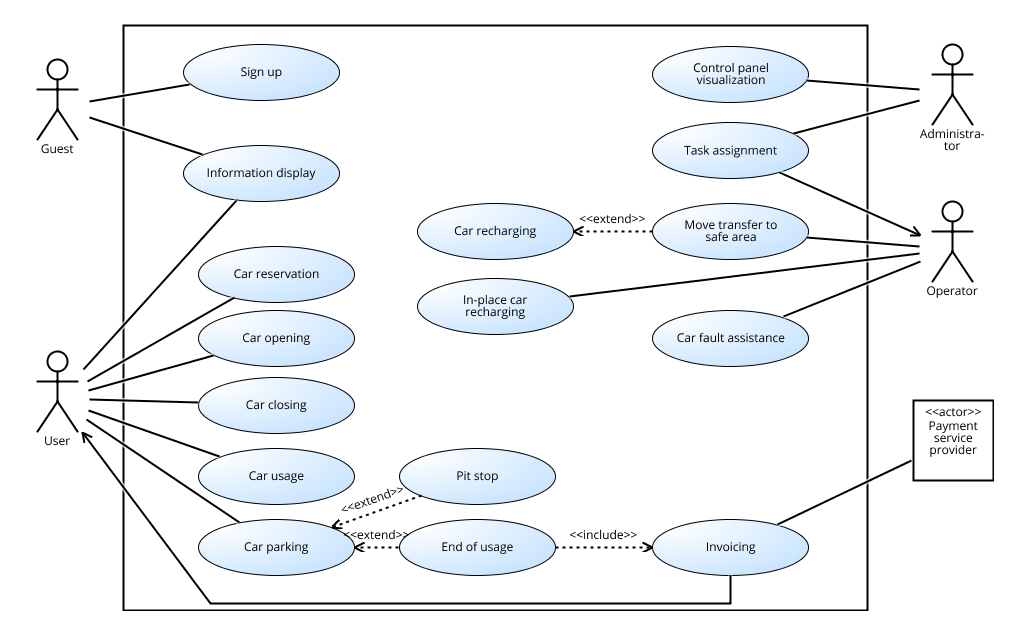
\includegraphics[width=\textwidth]{img/use_case.png}

	\subsubsection{Use case 1: Reserve a car}
		\begin{description}
			\item[Name] Reserve a car
			\item[Actors] \hfill
				\begin{description}
					\item[User] The user who wants to reserve a car.
				\end{description}
			\item[Entry condition] The user decides to reserve a car to take within the next hour.
			\item[Flow of events] \hfill
				\begin{enumerate}
					\item The user logs in into the mobile app and goes to the reservation section. 
					\item The system automatically retrieves and displays the location of the user, but the user can specify a different location if needed.
					\item The system displays the position of the available cars close to the selected location.
					\item The user selects a car and confirms the reservation.
				\end{enumerate}
			\item[Exit condition] The system reserves the car for the user.
			\item[Exceptions] \hfill
				\begin{itemize}
					% \item \textbf{The system is not able to locate the user automatically.} The user is required to insert a position manually.
					\item \textbf{The system is not able to find a position inserted manually.} The user is informed and the operation is aborted.
					\item \textbf{There are no available cars.} The user is informed and the operation is aborted.
					\item \textbf{The user cancels the operation before confirming.} The reservation process is not completed and the car remains available to other users.
					\item \textbf{The user doesn't come get the car before one hour.} The user is notified of the lost reservation. The system charges them the lost reservation fee. The car becomes available again.
				\end{itemize}
			\item[Special Requirements] None.
		\end{description}

	\subsubsection{Use case 2: Park in known safe area}
		\begin{description}
			\item[Name] Park in known safe area
			\item[Actors] \hfill
				\begin{description}
					\item[User] The user of the car.
					\item[Car] The car in use.
				\end{description}
			\item[Entry condition] The user is driving and has reached their destination. They know a safe area close to the destination.
			\item[Flow of events] \hfill
				\begin{enumerate}
					\item The safe area is free and the user parks in it.
					\item As the car is turned off, the system detects it is in a safe area.
					\item The user exits the car.
					\item The time windows starts.
					\item The system closes the car.
					\item The time window ends.
					\item The system charges the user for the ride.
				\end{enumerate}
			\item[Exit condition] The user leaves the car and the car becomes available to other users.
			\item[Exceptions] \hfill
				\begin{itemize}
					\item \textbf{The safe area is taken.} The user can't end their ride and this operation is aborted.
				\end{itemize}
			\item[Special Requirements] None. % TODO are there any?
		\end{description}

	\subsubsection{Use case 3: Park with money saving option}
		\begin{description}
			\item[Name] Park with money saving option
			\item[Actors] \hfill
			\begin{description}
				\item[User] The user of the car.
				\item[Car] The car in use.
			\end{description}
			\item[Entry condition] The user selects the \textit{money saving option} at some point of their ride and insert their destination.
			\item[Flow of events] \hfill
			\begin{enumerate}
				\item The system indicates the user the suggested safe area for their destination.
				\item The user parks in the suggested safe area.
				% from here, same as Use case 2:
				\item As the car is turned off, the system detects it is in a safe area.
				\item The user exits the car.
				\item The time window starts.
				\item The system closes the car.
				\item The time window ends.
				\item The system charges the user for the ride. A discount is applied for using the \textit{money saving option}.
			\end{enumerate}
			\item[Exit condition] The user leaves the car and the car becomes available to other users.
			\item[Exceptions] \hfill
			\begin{itemize}
				\item \textbf{The suggested safe area becomes taken while the user is driving.} The system selects another safe area and notifies the user of the new suggestion.
				\item \textbf{The user parks in another safe area.} The system notifies the user that they will not receive a discount. If the user decides to end the ride anyway and exits the car, the system charges them without applying the \textit{money saving option} discount.
				\item \textbf{The destination of the user changes.} The user selects a new destination and the system indicates another suggestion.
				\item \textbf{The user disables the \textit{money saving option} while driving.} The suggested safe area stops being displayed and the ride continues as normal.
			\end{itemize}
			\item[Special Requirements] The \textit{money saving option} must be selected before stopping the car in a parking area.
		\end{description}

	\subsubsection{Use case 4: Park in a recharging area}
		\begin{description}
			\item[Name] Park in a recharging area
			\item[Actors] \hfill
			\begin{description}
				\item[User] The user of the car.
				\item[Car] The car in use.
			\end{description}
			\item[Entry condition] The user is about to park in a recharging area.
			\item[Flow of events] \hfill
			\begin{enumerate}
				\item The user parks the car in the recharging area.
				% same as parking in safe area
				\item As the car is turned off, the system detects it is in a safe area.
				\item The user exits the car.
				\item The time window starts.
				\item The system closes the car.
				% same as parking in safe area
				\item The user plugs the car into the power grid through the supply point installed in the parking space.
				\item The system detects the car is recharging.
				\item The time window ends.
				\item The system modifies the charge applied to the user for the ride. A 30\% discount is applied to promote virtuous behaviors.
				\item The system charges the user for the ride.
			\end{enumerate}
			\item[Exit condition] The user leaves the car and the car becomes available to other users.
			\item[Exceptions] \hfill
			\begin{itemize}
				\item \textbf{The user does not plug the car into the power grid.} The user is charged as if they parked in a safe area.
				\item \textbf{The user plugs the car into the power grid after the time window has closed.} The user is invoiced the moment the time window closes. The user is charged as if they parked in a safe area.
			\end{itemize}
			\item[Special Requirements] The user plugs in the car during the time window after the ride. Otherwise the discount is not applied.
		\end{description}	
		
	%FIXME generalise?
	\subsubsection{Use case 5: Manually assist a parked car}
		\begin{description}
			\item[Name] Manually assist a car
			\item[Actors] \hfill
				\begin{description}
					\item[Admin] The administrator who sends the operator.
					\item[Operator] The operator sent to recover the car.
				\end{description}
			\item[Entry condition] The administrator is notified by the system that a parked car needs manual assistance.
			\item[Flow of events] \hfill
				\begin{enumerate}
					\item The admin checks the issue the system is displaying. It can be one of the following:
						\begin{itemize}
							\item the car is in a safe area without enough power charge to be used;
							\item the car is in a recharging area without the plug inserted.
						\end{itemize}
					\item The admin assigns the maintenance work to an operator.
					\item The operator accepts the assignment and the admin is notified of it.
					\item When available, the operator performs the \textit{maintenance operation} (see below).
					\item The operator checks the assignment as completed.
				\end{enumerate}
			\item[Exit condition] The maintenance activity has been performed and the admin is notified of the completion.
			\item[Exceptions] \hfill
				\begin{itemize}
					\item \textbf{The operator is not able to perform the maintenance.} The assignment is marked as \textit{not completed}, the cause is inserted into the system. The admin will be notified of it and will either assign the problem to another operator or manage it without the help of the system. The assignment will be anyway closed at the end of this process.
				\end{itemize}
			\item[Special Requirements] The operator cannot refuse an assignment if he is online and always accept it within a working day. An operator is always online when at work.
			The operator always marks the assignment as either \textit{completed} or \textit{not completed} before the end of the workday.
		\end{description}
		In the previous use case we refer to \textit{maintenance operation} as to one of the following:
		\begin{itemize}
			\item \textbf{Issue}: the car is in a safe area without enough power charge to be used. \textbf{Maintenance operation}: the car is towed to a recharging area and plugged into the power grid once there.
			\item \textbf{Issue}: the car is in a recharging area without the plug inserted. \textbf{Maintenance operation}: the car is plugged into the power grid.
		\end{itemize}
	

	\subsubsection{Use case 6: Manage infractions}
		\begin{description}
			\item[Name] Manage infractions
			\item[Actors] \hfill
				\begin{description}
					\item[Admin] The system administrator.
					\item[User] The user responsible for the infraction.
				\end{description}
			\item[Entry conditions] The company receives by mail the notification of the infraction.
			\item[Flow of events] \hfill
				\begin{enumerate}
					\item The company pays the fine for the infraction to the police.
					\item The admin logs into the system and inserts the license plate and the time of the infraction to find the responsible user.
					\item The system shows the name of the user.
					\item The system charges the user with the fine.
					\item The system notifies the user of the payment.
				\end{enumerate}
			\item[Exit conditions] The legal procedure has been closed and the user has paid the fine.
			\item[Exceptions] \hfill
				\begin{itemize}
					\item \textbf{The infraction causes the user to lose their license} The admin temporarily bans the user. The user won't be able to reserve a car anymore until they send another valid license via email to the admin.
				\end{itemize}
			\item[Special requirements] None.
		\end{description}

	\subsubsection{Use case 7: Assist user after an accident}
		\begin{description}
			\item[Name] Assist user after an accident
			\item[Actors] \hfill
			\begin{description}
				\item[User] The user driving the car.
				\item[Admin] The administrator who receives the notification from the system.
				\item[Operator] The operator sent to assist the user.
			\end{description}
			\item[Entry condition] The user is driving and is involved in an accident.
			\item[Flow of events] \hfill
			\begin{enumerate}
				\item The User notifies the Admin that an accident has happened. In case of serious accidents, it is the Accident Detection System of the car, instead of the User, that notifies the Admin. After the notification, the User waits for an Operator to arrive.
				\item The Admin dispatches an Operator with a tow-truck.
				\item The Operator arrives on site.
				\item The Operator manages the jointly-agreed statement for insurance purposes with other drivers involved and takes care of contacting the insurance company.
				\item When everything is done on site, the Operator takes the car to the company garage, to be analyzed by the insurance company if needed.
				\item The user leaves the site when the Operator takes the car away.
			\end{enumerate}
			\item[Exit condition] Eventually, the car is repaired and the insurance company emits a result on the accident report and refunds the company for the reparation costs of the car. The car is put back in use (the car is taken to a parking area; it can be reserved again).
			\item[Exceptions] \hfill
			\begin{itemize}
				\item \textbf{The User leaves the site before the removal of the car.} The Operator can report it to the system, and the user will be charged of an extra. If the User is penally implied in the accident, the Operator provides their personal details to the law enforcement.
				\item \textbf{The insurance asserts that the accident is fault of the User and doesn't take responsibility for it.} The User is fully charged of the reparation costs.
			\end{itemize}
			\item[Special Requirements] The Operator cannot refuse to be assigned to an accident if he is online and always accept it within 10 minutes. An Operator is always online when at work.
			The Accident Detection System always detects an accident when the User is unconscious. If the accident detection system detects an accident and the user is conscious, it is the detection system who alerts the system of the accident. The system then prevents the user to send another notification. 
		\end{description}

	\subsubsection{Use case 8: Assist a user on-site after a car breakdown}
		\begin{description}
			\item[Name] Assist user after a car breakdown
			\item[Actors] \hfill
			\begin{description}
				\item[User] The user driving the car.
				\item[Admin] The administrator who receives the notification from the system.
				\item[Operator] The operator sent to assist the user.
			\end{description}
			\item[Entry condition] The user is driving and notices a car breakdown. An empty battery while driving is considered as a car breakdown.
			\item[Flow of events] \hfill
			\begin{enumerate}
				\item The User notifies the Admin that a breakdown has happened. After the notification, the User waits for an Operator to arrive. The charges for the User are suspended.
				\item The Admin dispatches an Operator.
				\item The Operator arrives on site.
				\item The Operator repairs the car.
				\item Once the reparation has ended, the User is assigned again to the car and the charges start again.
			\end{enumerate}
			\item[Exit condition] The Operator marks the assignment as \textit{completed} and leaves. The User is back on their car.
			\item[Exceptions] \hfill
			\begin{itemize}
				\item \textbf{The Operator decides that the reparation can't be done on-site.} The use case \textit{Assist a user with a not on-site reparation} is invoked.
				\item \textbf{The User leaves the site before the reparation ends.} The Operator reports it to the system. At the end of the reparation, the User is not assigned to the car anymore and is invoiced for the ride (until the breakdown occurred). The Operator notifies the Admin that the car must be taken to a parking area and leaves the site. The Admin dispatches an Operator with a tow truck. The new Operator takes the car to the closest available parking area.
				\item \textbf{The Operator asserts that there is no need for intervention and the User is still on site.} The User is fined. The car is assigned to the User again and the charges start again.
				\item \textbf{The Operator asserts that there is no need for intervention and the User has gone from the site.} The User is fined. The Operator notifies the Admin that the car must be taken to a parking area and leaves the site. The Admin dispatches an Operator with a tow truck. The new Operator takes the car to the closest available parking area.
			\end{itemize}
			\item[Special Requirements] The Operator cannot refuse an assignment if he is online and always accept it within 10 minutes. An Operator is always online when at work.
		\end{description}

	\subsubsection{Use case 9: Assist a user with a not on-site reparation}
		\begin{description}
			\item[Name] Assist a user with a not on-site reparation
			\item[Actors] \hfill
			\begin{description}
				\item[User] The user driving the car.
				\item[Admin] The administrator who receives the notification from the system.
				\item[Operator] The operator sent to assist the user.
			\end{description}
			\item[Entry condition] The operator sent to fix a breakdown asserts that the reparation can't be done on-site and notifies the Admin of the change. The notification contains a brief description of the reason.
			\item[Flow of events] \hfill
			\begin{enumerate}
				\item The User is not assigned to the car anymore and is invoiced for the ride (until the breakdown occurred). The car cannot be reserved anymore.
				\item The Admin dispatches a new Operator with a tow truck.
				\item The new Operator contacts the insurance company and notifies the breakdown.
				\item The new Operator takes the car to the company garage.
			\end{enumerate}
			\item[Exit condition] Eventually, the car is repaired and the insurance company emits a result on the accident report and refunds the company for the reparation costs of the car. The car is put back in use (the car is taken to a parking area; it can be reserved again).
			\item[Exceptions] \hfill
			\begin{itemize}
				\item \textbf{The insurance asserts that the accident is fault of the User and doesn't take responsibility for it.} The User is fully charged of the reparation costs.
			\end{itemize}
			\item[Special Requirements] The new Operator cannot refuse the assignment if he is online and always accept it within 10 minutes. An Operator is always online when at work.
		\end{description}
